\chapter{线性代数 - 线性方程组}

\begin{figure}[ht]
  \centering
  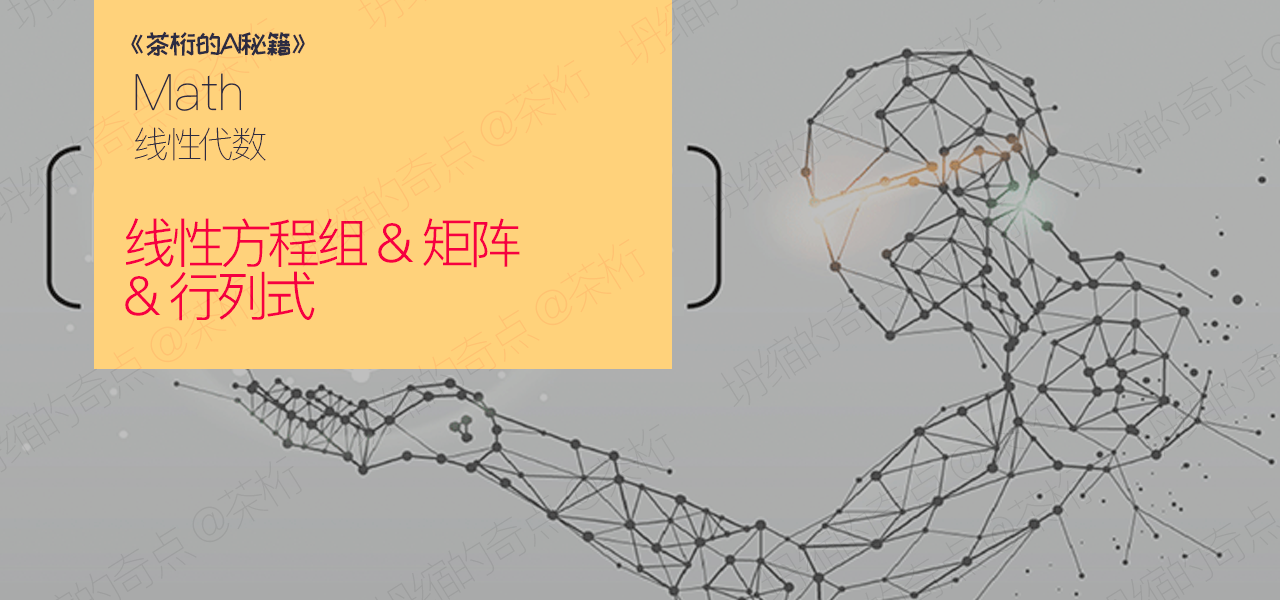
\includegraphics[width=1\linewidth]{asset/20230905111111.png}
\end{figure}

\newpage

结束了「微积分」部分的学习之后我们稍作休整, 今天正式开始另外一部分: 「线性代数」的学习. 小伙伴们放松完回来要开始紧张起来了. 

之前说过, 不管是哪一个工程学科, 根基都在于数学. 所以不管是做什么, 你都得了解一定的数学知识. 只是不同的领域对数学的运用精尖程度不一样. 比如说, 金融领域对于数学的要求就会比较高, 但是也有一些学科, 比如说绘画什么的, 对数学要求就会不那么高. 

对于人工智能, 所需要的数学知识在导论第一节课我给大家列过一个目录, 基本也就是目录上的那些内容, 那些就是我们最核心的点. 

有些同学可能会觉得导论课很简单, 确实, 人工智能直接运用的那一些东西就那么点, 在这一部分知识的背后, 它有一个庞大的数学体系. 所以, 上一部分「微积分」大家应该也发现了, 这个知识体系非常庞大, 各方面都有一环套着一环. 

当然, 这其中有部分技术比较差的同学, 看那些公式会觉得头晕. 但其实别担心, 这个问题并不是很大, 因为知识点就这么多, 我都列的很清楚, 针对性的自己再去提升一下, 妥妥的. 

咱们现在要学的部分是「线性代数」, 这一部分非常重要, 其中矩阵形式是在人工智能里面包括神经网络主要的一种数据的载体形式. 也就是说, 数据是怎么进入神经网络里面被处理的, 以及出来的这些结论是一种什么样的形式呈现出来的, 答案就在矩阵里, 或者说是「向量」. 

所以这部分是一个非常基础, 非常重要的一部分内容. 好消息是, 难度相对来说并没有特别的大, 当然, 我说的是矩阵这一部分本身非常简单, 如果要想学到一些比较难的内容, 建议大家可以去看看高等代数的相关教材. 那部分的难度会让你怀疑人生.

在人工智能里并没有必要学那么深, 至于是否需要去补充额外的书籍, 咱们这样判断, 如果课程里的内容都能消化吸收, 也都能完全理解, 那就没必要去看了, 没那个必要. 如果你需要进一步的查阅资料, 在我课程中遇到了一些难点无法理解, 可以去找其他书籍来对照着理解. 

\section{线性方程组}

不知道大家对于导论里面的内容还记得多少, 我们曾在里面介绍过线性代数, 介绍过其相关背景. 

在我国古代几千年前, 其实就有一些关于线性代数或者说线性方程组的一些问题了. 比如说导论提到过的「鸡兔同笼」问题. 这个是「孙子算经」里的问题, 而且这部分的内容在导论课里面也给大家讲过, 非常简单, 可能也就相当于小学的一个水平吧. 

只要按照现代的方程思想你把未知量设出来, 然后列好线性方程组, 去做出来就可以了. 慢慢的你就通过一些消元法, 把最终的解求出来. 

人们在现实生活当中, 在日常生活生产、经济活动当中遇到了非常多关于线性方程组的一类问题. 

线性方程组长什么样?来看一下: 

\begin{align*}
  \begin{cases}
    a_1x_1 + b_1x_2+ c_1x_3 + d_1x_4 = e_1 \\
    a_2x_1 + b_2x_2+ c_2x_3 + d_2x_4 = e_2 \\
    a_3x_1 + b_3x_2+ c_3x_3 + d_3x_4 = e_3 \\
    a_4x_1 + b_4x_2+ c_4x_3 + d_4x_4 = e_4 \\
  \end{cases}
\end{align*}


它有一系列的未知量, 我们一般用x和其下标来表示$x_1, x_2, x_3$.  还有一些系数, 每一个未知量前面都有系数, 这些方程的右边还有一些常数. 

\section{矩阵}

久而久之人类就发现, 这东西是有一定规律的. 求解这些方程组是有一定的套路、有一定规律的, 所以慢慢的人类就变得聪明起来了, 就把线形方程组给它去做了一个抽象, 把系数以及它的常数给抽象出来, 形成了这么一个矩阵的东西:

\begin{align*}
\begin{cases}
a_1x_1 + b_1x_2+ c_1x_3 + d_1x_4 = e_1 \\
a_2x_1 + b_2x_2+ c_2x_3 + d_2x_4 = e_2 \\
a_3x_1 + b_3x_2+ c_3x_3 + d_3x_4 = e_3 \\
a_4x_1 + b_4x_2+ c_4x_3 + d_4x_4 = e_4 \\
\end{cases}
\quad \Longrightarrow \quad
\begin{bmatrix}
a_1 \quad b_1 \quad c_1 \quad d_1 \quad e_1 \\
a_2 \quad b_2 \quad c_2 \quad d_2 \quad e_2 \\
a_3 \quad b_3 \quad c_3 \quad d_3 \quad e_3 \\
a_4 \quad b_4 \quad c_4 \quad d_4 \quad e_4 \\
\end{bmatrix}
\end{align*}


在导论课里面, 我问过大家线形方程组是由什么东西唯一确定. 判断一个线型方程组和另外一个线型方程组之间不同, 是根据什么判断的. 是对于未知量的表示符号选取的不同吗?一个里面是x一个里面是y?不是, 其实未知量用什么字母去表示没有任何意义, 甚至说用中文字符用日语字符去表示都OK, 它们其实是\textbf{由「系数唯一确定」} 的. 

这也是为什么我们抽象的时候其实没有太关心这些未知量的符号, 只是把这些系数以及常数给它提取了出来, 就把抽取出来的东西叫做矩阵. 

矩是正正方方的意思, 阵就是一种排列. 

对于我们一开始所见到的线形方针组, 可以简化成这种形式:

\[
  Ax = b
\]

以上, 用矩阵的形式去简化. 在这个式子中, 每一个字母代表了不同的意义, $A$: 系数矩阵, $x$: 未知量向量, $b$: 常数向量. 具体说来, 就是如下的这种表示: 


\begin{align*}
  A = 
  \begin{bmatrix}
  e_1 \quad b_1 \quad c_1 \quad  d_1\\
  e_2 \quad b_2 \quad c_2 \quad  d_2\\ 
  e_3 \quad b_3 \quad c_3 \quad  d_3\\
  e_4 \quad b_4 \quad c_4 \quad  d_4\\
  \end{bmatrix}, \quad
  x = 
  \begin{bmatrix}
  x_1 \\
  x_2 \\
  x_3 \\
  x_4
  \end{bmatrix}, \quad
  b = 
  \begin{bmatrix}
  e_1 \\
  e_2 \\
  e_3 \\
  e_4
  \end{bmatrix}
\end{align*}


在这之后, 我们来认识一下比较独特的一种运算, 这种运算是针对某一种特别的矩阵所提出来的. 这种比较特别的矩阵叫做方阵, 方阵就是行数等于列数, 可以把它想象成正方形矩阵, 行数和列数都是相等的. 

\section{行列式}

对于方阵(行数=列数), 我们定义了一种特别的运算--行列式: 

\begin{align*}
  A = 
  \begin{bmatrix}
  e_1 \quad b_1 \quad c_1 \quad  d_1\\
  e_2 \quad b_2 \quad c_2 \quad  d_2\\ 
  e_3 \quad b_3 \quad c_3 \quad  d_3\\
  e_4 \quad b_4 \quad c_4 \quad  d_4\\
  \end{bmatrix}, \quad
  |A| = 
  \begin{vmatrix}
  a_1 \quad b_1 \quad c_1 \quad d_1\\
  a_2 \quad b_2 \quad c_2 \quad d_2\\
  a_3 \quad b_3 \quad c_3 \quad d_3\\
  a_4 \quad b_4 \quad c_4 \quad d_4\\
  \end{vmatrix}
\end{align*}

就在矩阵的外面加一个像绝对值符号的两个竖线, 然后他展开的写法也是两个竖线, 和平时矩阵的表示方法不太一样. 

它的运算是怎么样去进行的?首先我们来看一个比较简单一点的. 

\begin{align*}
  \begin{vmatrix}
  a \quad b \quad c \\
  x \quad y \quad z \\
  r \quad s \quad t
  \end{vmatrix}
\end{align*}

有些小伙伴可能会在其它的一些资料上面, 或者过往的学习经历当中都有提到过. 

这里是一个3阶的. 3阶的可能还稍微复杂一点, 我觉得还是有必要跟大家先走一遍二阶的, 我们就先只看左上角的部分吧. 

\begin{align*}
  \begin{vmatrix}
  a \quad b  \\
  x \quad y  \\
  \end{vmatrix}
  =
  ay - bx
\end{align*}

二阶的, 就用a乘以y, 再减去b乘以x就可以了. 其实就是对角线相乘, 再用主对角线的乘积减去副对角线上的乘积. 一般在矩阵中, 我们把左上到右下的这一条对角线称为主对角线, 右上到左下的这条对角线称为副对角线. 

我们再回过头来看$3 \times 3$的行列式该如何计算, 它其实也是对角线相加然后再相减, 道理是一模一样的. 

\begin{align*}
  \begin{vmatrix}
  a \quad b \quad c \\
  x \quad y \quad z \\
  r \quad s \quad t
  \end{vmatrix}
  =
  ayt + bzr + cxs - azs - bxt -cyr
\end{align*}

先来看主对角线, 对角线上是$ayt$, 然后看$b$,  与主对角线同一方向的, 就是$bz$, 第三行上没有了, 那我们就往前找, 去找第一列, 所以最后就是$bzr$, 那么$c$也是一样的道理, 就是$cxs$. 然后我们把这三个相加, 因为和主对角线方向是一致的, 得到$ayt + bzr + cxs$. 

然后我们来看副对角线上, 副对角线是从右上到左下, 那么如果从$a$开始的话, $a$左侧没有列, 那就到后面去找, 就是$azs$, 然后$b$呢, 就是$bxt$, 接着是$cyr$, 然后也将它们进行相加. 就是$azs+bxt+cyr$. 

之后, 就和二阶一样, 我们用主对角线上的值减去副对角线上的值, 那么就变成: 

\begin{align*}
  (ayt + bzr + cxs) - (azs+bxt+cyr) \\
  = ayt + bzr + cxs - azs - bxt -cyr
\end{align*}

它的结果就是这样去进行计算. 

三阶的也是比较简单的. 三阶、二阶我们都知道怎么样去做了, 可是我们在实际工程项目或者说工程问题里面, 行列式阶数非常的高, 可以说甚至是几十万行乘几十万列的、几百万乘几百万的都有. 那你就不是按照什么主对角线相加, 减去副对角线这样子了. 所以阶数更高我们怎么样计算?

我们要先来了解一下概念, 这些概念, 待会我们的讲解都需要用到, 所以大家要认真听. 

\subsection{全排列和逆序数}

\textit{全排列} 这个概念应该是大家在高中数学里面有学到过, 它表示什么意思?就是我有n个不同的元素, 然后把n个不同的元素给它排列起来有多少种不同的排列方式. 所有的这些不同排列方式的总和加在一起有多少种?

后来一些推算发现它排列的数量应该是这个样子的: 

\[
  P_n = n \times (n-1) ... 2 \times 1 = n!
\]

就是我们把全排列的数量用$P_n$来表示, 它等于$n$乘上$n-1, n-2, n-3...$一直乘到$2$,乘上$1$. 那最后等号后面的东西我们在之前的课程当中也介绍过, 它叫做阶乘. 

阶乘就是从1一直乘到n这个数, 中间是递增1的, 所以被称为阶乘. 

阶乘大家不要看它感觉好像很很普通, 感觉像是一个二次函数一样, 类似于$n^2$这样, 其实n的阶乘比2的n次方增长的速度还要快, 是增长非常快的一种数. 只不过平常咱们用的也不是特别多, 大家也感受不到. 

「全排列」这个概念之后, 我们来了解第二个概念:\textit{逆序数}. 逆序数的概念是: 对于一个排列, 标准顺序规定为从小到大, 大数在小数前面就称为逆序. 一个排列中逆序的数目称为逆序数, 用希腊字母$\tau$来表示(读作$\mathord{tau}$). 

下面来看一个例子: 

\begin{align*}
  \tau (53214) = 4+2+1 = 7
\end{align*}

这个式子怎么理解呢?我们一个一个来看. 

首先我们看在这个数列中, $5$似乎应该是最大的, 所以按顺序应该是排在最右面, 但是它排在了前面, 分别比$3,2,1,4$大, 那么它产生了\textcolor{red}{4}个逆序.

再来看数值$3$,  $3$比$2, 1$大, 但是比$4$小, 就应该在$4$前面, 所以产生了\textcolor{red}{2}个逆序.

然后是$2$, 它比$1$大, 但是比$4$小, 产生了\textcolor{red}{1}个逆序. 

再来看$1$,  $1$比$4$小, 就应该在$4$前面, 所以就没有逆序, 那最后一个4后面没数字了也没有比较了, 也没有逆序. 

所以最后就是\textcolor{red}{$4 + 2 + 1 + 0 + 0$}, 也就是\textcolor{red}{$4 + 2 + 1$}, 得到了数值\textcolor{red}{7}. 

所以逆序数它没有什么很神秘的地方, 也就这么一回事. 就是算你有几个成天想造反的数, 那些小头目一天到晚的想往后躲, 还想让老板冲锋陷阵到第一线顶在前面, 这肯定是不行的. 所以把它称为逆序. 通过这个例子我们就能知道逆序数是怎么一回事. 

\subsection{N阶行列式}

我们来看一下对于任意一个N阶的行列式的一个求解. 在教科书上面规定的一种所谓的解法如下: 

\begin{align*}
  \begin{vmatrix}
  a_{11} \quad \cdots a_{1n} \\
  \vdots \quad \ddots \quad \vdots \\
  a_{n1} \quad \cdots \quad a_{nn}
  \end{vmatrix}
  = 
  \sum_{p_1p_2...p_n} (-1)^{\tau(p_1p_2...p_n)}a_{1p_1}a_{2p_2}...a_{np_n}
\end{align*}

解释一下的话, 就是说我这里总共是n行乘n列, 叫做n阶. 行列式都是针对方正而言的, 方正行列数目都是相等的, 所以是n行n列. 

我们需要知道, 真正的实际生活当中或者说工程运用里面没有谁是真的用式子去去求解的. 这里只不过告诉大家这是一个什么东西. 如果真的其他什么办法都没有了, OK那你回过头来看一下这里的式子. 

其实在很多科学概念里面都是一样, 就是包括汉语词典、英语词典也是一样. 你们翻汉语词典、英语词典时候会有一种感受, 就是看它那个解释, 我们在日常生活当中是不会那样解释的. 但是那种解释为什么是很明显的字典体, 目的最主要的不是用通俗化的语言向别人解释这些字是什么意思, 其实更多的是一种归纳整理的目的. 

说回正题, 式子代表了什么意思?这里每一个元素下面都有两个下标, 我们之前也说过, 分别是代表行和列. 比如$a_{n1}$, 就是代表第n行第1列, 同理, $a_{nn}$就是代表第n行第n列. 

等号后面的部分有三个部分组成, 一个是$\Sigma$, 一个是$(-1)^{\tau(p_1p_2...p_n)}$, 算逆序数的这么一个数. 最后是$a_{1p_1}$乘上$a_{2p_2}, ...$,  一直乘乘乘, 乘到$a_{np_n}$. 

首先我们说一下第三项是什么意思, 第三部分它代表了每一行挑一个数, 比如$a_{1p_1}$就是第一行, 先别管这$p_1, p_2$是多少, 只看前面的下标的数字. $a_{1p_1}$它表示第一行,$a_{2p_2}$是第二行,..., $a_{np_n}$它表示第n行, 所以我们从行来看就是每一行挑一个数. 

然后每一行挑的数它不能是同一列的. 比如说我$p_1$值等于1的话, 那它就代表了$a_{11}$,  那后面的数就不能取同一列的了, 也就是不能是$a_{2p_1}$, 必须等于其他数, 比如说$2p_2$, $2p_3$代表着是第二列第三列. 那其实也就是说, 这些数字必须是不同行, 并且不同列的数. 

把能想出来的所有的这些排列给他找出来, 这里我选择沿着对角线这样选. 

第一行我选$a_{11}$, 第二行我选$a_{22}$, 第三行我选$a_{33}$, 这样子也是一种选法. 那不就得到了一个关于 $p_1, p_2, ..., p_n$ 的一个排列了吗. 

现在就可以说到第二项了, 第二项里它的排列就是$1, 2, 3$, $1, 2, 3$里面并没有逆序, 逆序数上就是0. 所以$\tau(p_1p_2...p_n)$在这里就是0. 

$-1^0$代表了什么?就是1. 

是不是任意时候$(-1)^{\tau(p_1p_2...p_n)}$都是1呢?并不是, 要看逆序数的结果. 刚才我说过了, 把能想出来的所有的这些排列都找出来, 我举例仅仅是一种而已. 那我$p_2$可以是其他的列么?当然可以, 如果我这次选择$P_2$是$p_3$,  $p_3$是$p_2$, 其他都不变, 则此时的逆序数就变成$1$了. 因为$3$在$2$前面是逆序, 并且只有这一个逆序. 

此时, $(-1)^\tau$的结果, 就变成了-1. 

到这里大家就能明白了, 这个逆序数为指数的$(-1)^\tau$, 要么是+1, 要么是-1, 那其实就说要么加, 要么减. 

当我把所有情况都给找出来算一遍, 然后把这些结果全部给它加在一起, 就得到了行列式的一个值. 

到这里为止这些东西绕吗?还好吧?假如还有不理解的, 可以回过头再多看几遍. 

为什么行列式是这样子去定义它的解法?一般来说, 在中学或者大学里面的时候我们想去证明一些题或者去解一些题, 往往发现定义法它是最没用的一种方法, 或者可以说成是给我们的助力最小. 

来吧, 接下来我来讲讲到底我们实际上是怎么样去得到矩阵对应的行列式结果. 

其实主要是有两种方法: 

\begin{enumerate}
  \item 第一种是把矩阵转化成上三角或下三角矩阵. 
  \item 第二种是将高阶行列式拆分成二阶 $/$ 三阶行列式. 
\end{enumerate}

先来说第一种, 三角矩阵. 

三角矩阵是方形矩阵的一种, 其特性就是非零系数的排列呈三角形状. 三角矩阵分为上三角矩阵和下三角矩阵两种, 其中上三角矩阵主对角线左下方的系数全部为0,  下三角矩阵则相反, 数主对角线右上方的系数全部为0.

拿一个行列式来打个比方: 

\begin{align*}
  \begin{vmatrix}
    a \quad b \quad c \\
    x \quad y \quad z \\
    r \quad s \quad t
  \end{vmatrix}
\end{align*}

$a, y, t$以及$b, c, z$它都是大于$0$的, 或者说非$0$的数. 而$x, r, s$它三个值都等于$0$. 这样看上去, 非$0$的这些数就形成了一个三角形. 我们把它叫做三角矩阵. 

为什么要把它弄成这样?因为它有一个非常好的特点, 就是只要我们能把$xrs$通过矩形变换把它弄成0, 对应的行列式的值有个非常美妙的性质, 就等于主对角线上元素的乘积. 它就和$bcz$没有任何关系了. 行列式的值就等于$a \cdot y \cdot t$. 所以这也是为什么我们想通过把矩阵转换成一个三角阵去求它的一个目的. 

因为此时矩阵所对应的行列式的值就恰好等于主对角线上面的元素的乘积. 

第二种方法是我们把高阶行列式拆分成二阶或者三阶的行列式, 就是通过余子式法之类的方法. 这里不和大家去细说了, 有兴趣的可以查找一下相关的书籍仔细学习下. 因为其实也没有必要, 你们只需要知道有这样一种方法, 是做什么的就可以了. 

也就是说, 行列式的求法是这么定义的没错, 但是现实当中没人真的这么去干. 这样去求话简直就是要人性命, 效率很低. 

知道实际上是怎么样求就OK了, 以及行列是是怎么样的一个东西. 

\section{(非)齐次线性方程}

接着, 说完行列式, 再介绍一个概念. 

我们对于线性方程组做一个分类, 就比如什么叫齐次线性方程组. 

比如我们本文开头的那个线性方程组: 

\begin{align*}
\begin{cases}
  a_1x_1 + b_1x_2+ c_1x_3 + d_1x_4 = e_1 \\
  a_2x_1 + b_2x_2+ c_2x_3 + d_2x_4 = e_2 \\
  a_3x_1 + b_3x_2+ c_3x_3 + d_3x_4 = e_3 \\
  a_4x_1 + b_4x_2+ c_4x_3 + d_4x_4 = e_4 \\
\end{cases}
\end{align*}

打比说, 我们这里的常数项($e_1, e_2, e_3, e_4$),  它全部为0. 我们就把它称作齐次线性方程组. 

什么叫非齐次线性方程组呢?也就是常数项不全为0, 至少有一个不等于0. 那就可以称为一个非齐次线性方程组. 

为什么叫齐次或者非齐次?其实不用特别去关心这个, 只是一种命名而已, 大家不用特别的去在意. 因为这也是初学者容易陷入的一个陷阱, 往往就被这些名字给唬住了. 如果真正理解了这些表面的字面意思所代表的真实含义是什么东西的话, 会发现根本没必要去管他叫什么东西. 

好, 在导论课里面和本文开头我们都强调了, 矩阵是由线性方程组抽象得来的. 那么现在的问题就是: 既然我们已经抽象出来了, 有没有一种比较好的办法去解线性方程组?那不然我们抽象有什么意义呢?下节课, 我们来了解下「克拉默法则」. 